\RequirePackage{plautopatch}
\documentclass[a4paper,12pt,dvipdfmx]{jlreq}
%英語フォント
\usepackage{tgtermes,tgheros,tgcursor}
%日本語を多書体にする
\usepackage{jlreq-deluxe}
%数式用
\usepackage{amsmath}
\usepackage[varg]{newtxmath}
\newcommand{\symbb}{\vvmathbb}
%日本語太字を戻すためのおまじない
\renewcommand{\bfdefault}{bx}
%図のとりこみ
\usepackage{graphicx}
\usepackage{physics}
%文献
\usepackage{hep-bibliography}
\bibliography{ref.bib}

\usepackage{tcolorbox}
\tcbuselibrary{breakable, skins, theorems}
%\usepackage{cleveref}

% font warningを出さないため
% \DeclareFontShape{JY2}{hgt}{b}{n}{<->ssub*hgt/bx/n}{}
% \DeclareFontShape{JY2}{hgt}{m}{it}{<->ssub*hgt/m/n}{}
% \DeclareFontShape{JT2}{hgt}{b}{n}{<->ssub*hgt/bx/n}{}
% \DeclareFontShape{JT2}{hgt}{m}{it}{<->ssub*hgt/m/n}{}

\newenvironment{myquote}{\begin{tcolorbox}[
  colback = blue!5, after = \noindent] }{\end{tcolorbox}}
\newenvironment{important}{\begin{tcolorbox}[
  colback = white,
  colframe = red!35,
  boxrule = 2mm,
  fonttitle = \bfseries,
  after = \noindent] }{\end{tcolorbox}}
\newenvironment{mycite}{\\ \qquad \textbullet\ }{\\}


\newcommand{\Zb}{\mathbb{Z}}
\newcommand{\Kt}{\widetilde{K}}
\newcommand{\ZIs}{Z_{\mathrm{Ising}}}
\newcommand{\ZGIs}{Z_{\mathrm{Ising}/\mathbb{Z}_2}}
\newcommand{\deltamod}{\delta^{\mathrm{mod}\ 2}}

\begin{document}

\begin{center}
  \textbf{\sffamily \LARGE 2次元Ising模型のKramers-Wannier双対性}
\end{center}

\begin{flushright}
  \textbf{\sffamily \Large 山口 哲}  
\end{flushright}

\section{導入}
このノートでは、2次元Ising模型のKramers-Wannier (KW) 双対性\cite{Kramers:1941kn,Kramers:1941zz}の導出をまとめている。もちろん、KW双対性の導出は、詳細な統計力学の教科書にも掲載されている\footnote{例えば\cite{itzykson1991statistical,Nishimori}など。}。それにもかかわらず、このノートで改めてまとめることにしたのは、熱力学極限だけでなく、精密な双対性についても論じたかったからである。Ising模型の相転移点の決定に際しては、熱力学極限だけで充分である。しかし、最近のトポロジカルな議論に用いる場合には、離散対称性のゲージ化に関する詳細な議論が求められる。本ノートでは、そのような観点も含めて導出を行う。

Ising模型について述べる。2次元の正方格子を考える。ここでは有限の格子で、トーラス状に周期境界条件が課されているとする。各サイトをラベル$i,j$で示す。各サイトには「スピン」の自由度$a_{i}=0,1$を置く。各リンクは両端のサイトのラベル$i,j$を用いて$\expval{ij}$のように表す。定数パラメーターを$K>0$と定めると、Ising模型の分配関数は以下の通りである。
\begin{important}
\begin{align}
\ZIs(K)=\sum_{{a}} \exp\left(
K\sum_{\expval{ij}:\text{すべてのリンク} }(-1)^{a_i+a_j}
\right).\label{Ising}
\end{align}
\end{important}
ここで$\sum_{{a}}$はすべてのスピン配位についての和を指す。パラメーター$K$は「逆温度」と呼ぶこととする。\footnote{厳密には、本当の逆温度を$\beta$、結合のパラメーターを$J$として$K=\beta J$である。ただし、これら二つのパラメーターは$K$の形でしか現れない。}

一方で、Ising模型の$\Zb_2$対称性をゲージ化した模型の分配関数は以下のようになる:
\begin{important}
\begin{align}
\ZGIs(K)=\frac12 \sum_{\text{boundary conditions}}
\sum_{{a}}\exp\left(
K\sum_{\expval{ij}:\text{すべてのリンク} }(-1)^{a_i+a_j}
\right)
\label{Ising/Z2}
\end{align}
\end{important}
ここで$\sum_{\text{boundary conditions}}$はトーラスの2つの周期の方向の境界条件を周期境界条件か反周期境界条件のどちらかを選ぶ4通りの境界条件についての和である。弦理論になじみのある方なら、「オービフォールド」の操作と理解することができるだろう。

Kramers-Wannier双対性の厳密な表式は、サイトの数を$V$とした場合、以下の通りである:
\begin{important}
\begin{align}
\frac{1}{(\sinh 2K)^{2V}}\ZGIs(K)=
\frac{1}{(\sinh 2\Kt)^{2V}}\ZIs(\Kt),\quad \sinh 2K \sinh 2\Kt=1
\label{KWduality}
\end{align}
\end{important}
ここでの因子$\frac{1}{(\sinh 2K)^{2V}}$は、作用の中に局所的な項として組み込むことが可能である。したがって、この式は二つの系の等価性を表している。このノートの目的は、この式の証明を与え、関連する事項について説明することである。

\section{Kramers-Wannier双対性の導出}
証明に関して次のような系を考える。まず、各リンク$\ell$に自由度$b_{\ell}=0,1$を置く。また、各プラケット$p$に自由度$c_{p}$を置く。その分配関数を
\begin{align}
  Z(K)=\sum_{\{b\}}\frac{1}{2^{V}} \exp\left[
    K\sum_{\ell:\text{links}}(-1)^{b_{\ell}}+i\pi\sum_{\substack{p=\expval{\ell_1 \ell_2 \ell_3 \ell_4}:\\ \text{plaquettes}}} c_{p}(b_{\ell_1}+b_{\ell_2}+b_{\ell_3}+b_{\ell_4})
  \right]
  \label{model1}
\end{align}
とする。$p=\expval{\ell_1 \ell_2 \ell_3 \ell_4}$はプラケット$p$を構成する4辺が$\ell_1, \ell_2, \ell_3, \ell_4$ということである。

方針としては、式\eqref{model1}を二つのやり方で変形したのが、大雑把に言って\eqref{KWduality}の左辺と右辺となる。

\subsection{第1の変形}
第1の変形では、まず$c$についての和を評価する。用いる式は整数$b$に対して 
\begin{align}
  \frac12\sum_{c=0,1}\exp(i\pi c b )
  =\deltamod_{b,0}
  :=
  \begin{cases}
    1& (b=0 \mod 2)\\
    0& (b=1 \mod 2)
  \end{cases}
  \label{deltamod}
\end{align}
という恒等式である。この式を用いると
\begin{align}
  Z(K)=\sum_{\{b\}}\sum_{\{c\}}\exp\left[
    K\sum_{\ell:\text{links}}(-1)^{b_{\ell}}
    \right]
    \prod_{\substack{p=\expval{\ell_1 \ell_2 \ell_3 \ell_4}:\\ \text{plaquettes}}} \deltamod_{b_{\ell_1}+b_{\ell_2}+b_{\ell_3}+b_{\ell_4}}
    \label{model1-1-1}
\end{align}
を得る。

式\eqref{model1-1-1}から、寄与が$0$でない$b_{\ell}$の配位は各サイトに置いたスピン$a_{i}$と「だいたい」1対1対応していることが次のように分かる。
\begin{itemize}
  \item 与えられた$a_{i}$の配位に対して$b_{\expval{ij}}=a_i-a_j \mod 2$とすれば、プラケットが$0$の$b$の配位が得られる。
  \item 逆にプラケットがすべて$0$である$b_{\ell}$の配位から次のようにして$a_{i}$の配位を得る。原点のサイト$0$を一つ固定する。図\ref{fig:path}のようにサイト$0$からサイト$i$までのリンク$\ell_1,\ell_2,\dots,\ell_N$を辿っていく経路をとり、
  \begin{align}
    a_{i}=a_{0}+b_{\ell_1}+b_{\ell_2}+\dots+b_{\ell_N} \mod 2
  \end{align}
  で与える。$b$のプラケットがすべて$0$なので、経路のプラケット1つ分の変形、そしてそれを繰り返して得られる変形で不変である。
\end{itemize}
\begin{figure}[htbp]
  \centering
  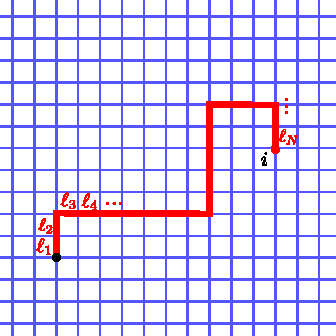
\includegraphics{path.pdf}
  \caption{{}}
  \label{fig:path}
\end{figure}

「だいたい」と言ったのは、次の2点で1対1対応では無いからである。
\begin{itemize}
  \item $b$の配位を決めたとき、$a_0$の値は任意である。つまり、$b$の配位を決めたとき、対応する$a$の配位は2種類ある。
  \item $b$から$a$を作るとき、経路によらないわけではない。プラケット1つ分の変形を繰り返すことでは繋がらない経路がある。この経路への依存性は、非自明なサイクルでの$b$の和の偶奇で特徴づけられる。逆に言えば、周期境界条件の$a$の配位からは非自明なサイクルでの$b$の和が偶数になる$b$の配位しか得られない。つまり、すべての$b$の配位と対応する$a$の配位は非自明なサイクルに関して周期境界条件あるいは反周期境界条件を持つものすべてを考えなければならない。
\end{itemize}
これらを正しく考慮すると
\begin{align}
  Z(K)=\ZGIs(K)\label{1st}
\end{align}
を得る。式\eqref{Ising/Z2}の$\ZGIs(K)$で全体にかかっている$1/2$が前者からくるもの、境界条件に関する和が後者から来るものである。

\subsection{第2の変形}
\label{sec:second}
\begin{figure}
  \centering
  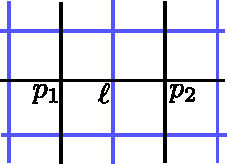
\includegraphics{link_plaquette.pdf}
  \caption{{}}
  \label{fig:link_plaquette}
\end{figure}

第2の変形では、\eqref{model1}で、まず$b$についての和をとる。1つのリンク$\ell$に注目し、$b_{\ell}$についての和を考える。$\ell$は図\ref{fig:link_plaquette}のように2つのプラケット$p_1,p_2$に共有されている。言い換えれば$\ell$に直交する双対格子のリンクが2つの双対格子のサイト$p_1,p_2$を繋いでいる。分配関数を$b_{\ell}$を含む因子に分けて
\begin{align}
  Z(K)=&\sum_{\{c\}}\frac{1}{2^V}\prod_{\ell}Z_{\ell}\\
  Z_{\ell}:=&\sum_{b_{\ell}=0,1}\exp\left[
    K(-1)^{b_{\ell}}+i\pi (c_{p_1}+c_{p_2})b_{\ell}
  \right]
  =e^{K}+(-1)^{c}e^{-K}
\end{align}
となる。ここで$c:=c_{p_1}+c_{p_2}$とした。これをさらに変形して
\begin{align}
  Z_{\ell}=2\cosh K (\tanh K)^{c}
  =\sqrt{2\sinh 2K}\ e^{\Kt(-1)^c}\label{Zelltemp}
\end{align}
となる。ここで$\Kt$は
\begin{align}
  \tanh K = e^{-2\Kt}
\end{align}
の式で定義した。ここから
\begin{align}
  \sinh 2 K \sinh 2\Kt =1 \label{dualK}
\end{align}
の式が導かれる。詳しい計算は付録\ref{sec:calculation}に書いておく。

これを用いると分配関数は次のように書かれる。
\begin{align}
  Z(K)&=\sum_{\{c\}}\frac{1}{2^V}\prod_{\ell}Z_{\ell}\notag\\
  &=\sum_{\{c\}}\frac{1}{2^V}\prod_{\ell=\expval{pq}}\sqrt{2\sinh 2K}\ e^{\Kt(-1)^{c_p+c_q}}\notag\\
  &=(\sinh 2K)^{V}\sum_{\{c\}}\prod_{\ell=\expval{pq}} e^{\Kt(-1)^{c_p+c_q}}\notag\\
  &=(\sinh 2K)^{V}\ZIs(\Kt).
\end{align}


\subsection{双対性のまとめ}

第1の変形の結果\eqref{1st}、$K,\Kt$の関係式\eqref{dualK}と合わせてKramerse-Wannier双対性の式\eqref{KWduality}が成り立つことが証明される。

\section{対称性と無秩序スピン}

この節では、KW双対性の周辺に出てくる事項、特に対称性と無秩序スピンについて解説する。

\subsection{ゲージ化されたIsing模型のゲージ不変な定式化}

ここでは、式\eqref{Ising}から始めて、ゲージ化されたIsingの作用をゲージ不変な形に書いておく。

Ising模型\eqref{Ising}に次のような操作をしてゲージ化する。
\begin{itemize}
  \item 通常の格子ゲージ理論と同様に各リンク$\ell$に$\Zb_2$の元$b_{\ell}$を配置する。
  \item $b_{\ell}$の作用は「プラケットの値が$0$」というものにする。これは通常のWilsonのプラケット作用で弱結合極限をとったものである。具体的には各プラケット$p=\expval{\ell_1 \ell_2 \ell_3 \ell_4}$に対して$\deltamod_{b_{\ell_1}+b_{\ell_2}+b_{\ell_3}+b_{\ell_4},0}$の重みをかける。さらにこれを式\eqref{deltamod}を用いて
  \begin{align}
    \deltamod_{b_{\ell_1}+b_{\ell_2}+b_{\ell_3}+b_{\ell_4},0}=\sum_{c_p=0,1}\frac{1}{2}e^{\pi i (b_{\ell_1}+b_{\ell_2}+b_{\ell_3}+b_{\ell_4})}
  \end{align}
  と書き換えておく。\footnote{このようなゲージ化を一般の格子ゲージ理論と区別して「トポロジカルなゲージ化」と呼ぶこともある。}
  \item ゲージ対称性を課す。ゲージ変換のパラメーターは各サイト$i$に置かれた$\lambda_i=0,1$である。リンク$\ell=\expval{ij}$上のゲージ場$b_{\expval{ij}}$とサイト$i$のスピン$a_{i}$はそれぞれ
  \begin{align}
    b_{\expval{ij}}'=b_{\expval{ij}}+\lambda_{i}+\lambda_{j},\quad
    a_{i}'=a_{i}+\lambda_{i}
    \label{gaugetransf}
  \end{align}
  と変換する。ゲージ変換で繋がっている配位は物理的に同じと考えるので、すべての配位を足し上げると$2^V$の数えすぎが生じる。これを解消するために、最後に分配関数を$2^{V}$で割っておく。
  \item Ising スピンとゲージ場の結合は通常の格子ゲージ理論と同様のである。つまり各リンクの重みを
  \begin{align}
    \exp\qty[K (-1)^{a_i+a_j+b_{\expval{ij}}}]
  \end{align}
  とする。これはゲージ不変である。
\end{itemize}

すべてまとめると、ゲージ化されたIsing模型の分配関数は
\begin{align}
  \ZGIs(K)=\sum_{\{a\}}\sum_{\{b\}}\sum_{\{c\}}\frac{1}{2^{2V}} \exp\left[
    K\sum_{\expval{ij}:\text{links}}(-1)^{a_i+a_j+b_{\expval{ij}}}+i\pi\sum_{\substack{p=\expval{\ell_1 \ell_2 \ell_3 \ell_4}:\\ \text{plaquettes}}} c_{p}(b_{\ell_1}+b_{\ell_2}+b_{\ell_3}+b_{\ell_4})
  \right]
  \label{model2}
\end{align}
となる。ここでゲージ固定$a_{i}=0$を行うと式\eqref{model1}になり、第1の変形の結果\eqref{1st}から\eqref{Ising/Z2}の形と同じになることが分かる。また前節の解析の結果から、これは逆温度が$\Kt$(式\eqref{dualK}参照)のIsing模型と(全体にかかる定数を除いて)同じである。

\subsection{様々な演算子}
式\eqref{model2}に含まれる自由度で書ける様々な自由度について考えよう。次の3種類について考える。
\begin{itemize}
  \item $c_p$から作るスピン演算子$\sigma_{p}=(-1)^{c_p}$
  \item $b_{\ell}$から作るWilsonループ演算子$\eta(C)=(-1)^{\sum_{k}b_{\ell_k}}$。ただし、$C$はリンク$\ell_1,\ell_2,\dots$から作られる閉じたループである。
  \item $a_i$から作るスピン演算子。$\mu_{i}\sim (-1)^{a_i}$
\end{itemize}

これらの演算子を作用\eqref{model2}の中だけで考えるなら、特に問題になることはない。その演算子の相関関数は通常どおり計算できる。これから考えたいのは上の演算子を、$a,b$の和をとってしまって得られる、$c$をIsing模型の中で考えることである。注意してほしいのは、$a,b$の和をとってしまったとしても、これらの演算子が無くなるわけではない。作用に出てくる場の関数として書けなくなるだけである。

スピン演算子$\sigma_{p}=(-1)^{c_p}$については、$a,b$を積分してしまった後も特に注意することはない。Ising模型に出てくるスピン変数で、相転移の秩序変数となる重要な演算子である。

$\eta$と$\mu$については注意が必要なので、以下で順に見ていく。


\subsection{対称性欠陥}

今考えている理論では、$b$のプラケットをすべて$1$にしているので、Wilsonループ$\eta(C)$は$C$をプラケット1個分変形しても値を変えない。このような性質を「トポロジカル」であるという。

トポロジカルな演算子(欠陥)は、(一般化)対称性を記述する。$\eta$が、$\sigma$スピンの反転という普通の対称性を記述する欠陥であることが次のようにして分かる。プラケット$p$に演算子$\sigma_{p}=(-1)^{c_p}$を挿入し、それを囲む経路$C$をとって$\eta(C)$を挿入する。$\eta(C)$はトポロジカルなので、値を変えずに$p$のプラケットまで縮めることができる。作用\eqref{model2}を見ると、この$\eta$の挿入は、和を取っている変数の変換$c_p'=c_p+1$で吸収することができる。このとき$\sigma_{p}=(-1)^{c_p}=-(-1)^{c'_p}$となる。したがって、次のようなWard-Takahashi恒等式が成り立つ。
\begin{align}
  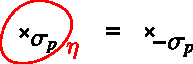
\includegraphics{wtz2.pdf}
\end{align}
これは、$\eta$が$\sigma$を反転する対称性欠陥であることを示している。

$a,b$を積分してしまった後で$\eta$がどのように表現されるか考えよう。$\eta(C)$を挿入した後で\ref{sec:second}項と同様に$a,b$を積分すると、$C$に含まれるリンクの相互作用に$(-1)$が余分にかかる。
\begin{align}
  \expval{\eta(C)\cdots}
  =\frac{1}{\ZIs}\sum_{\{c\}}\prod_{\ell=\expval{pq}} e^{\Kt(-1)^{c_p+c_q+\delta_{\expval{pq}}(C)}}\cdots
\end{align}
となる。ここで$\delta_{\ell}(C)$はリンク$\ell$が$C$と交わっていれば$1$、そうでなければ$0$という記号である。つまり、$C$と交わっているリンクは、相互作用が反強磁性に置き換わっている。この様子を図\ref{fig:z2defect}に示す。


\begin{figure}
  \centering
  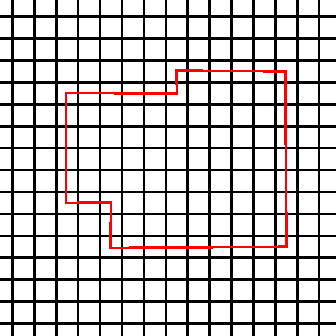
\includegraphics{z2defect.pdf}
  \caption{$a,b$の和をとってしまった後での対称性欠陥の様子。黒で表した格子には、サイトの上に通常のIsing模型のスピンがのっていてリンクに相互作用がのっている。赤で表した経路$C$は、各リンクと中点で直交するような線分で構成された経路である。$\eta(C)$の挿入は、$C$と交わるリンクの相互作用を大きさはそのままで、強磁性から反強磁性に置き換えたものである。}
  \label{fig:z2defect}
\end{figure}
\subsection{無秩序スピン}
式\eqref{model2}で表される模型でのサイト$i$に置かれた演算子$(-1)^{a_i}$について考えよう。まず重要なことは$(-1)^{a_i}$そのものはゲージ不変でないので、統計力学での良い演算子ではない。これが入った相関関数を考えると、いつでも$0$になってしまうのである。

\begin{figure}
  \centering
  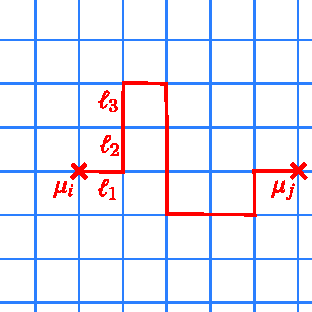
\includegraphics{disorder.pdf}
  \caption{赤い線が$\eta$線演算子で両端の$\mu_i,\mu_j$が無秩序スピン演算子である。この形でゲージ不変になっている。}
  \label{fig:disorder}
\end{figure}

これをゲージ不変にするために$\eta$線演算子($b$ Wilson line)をくっつけて
$\mu_i=(-1)^{a_i+b_{\ell_1}+b_{\ell_2}+\dots}$を考える(図\ref{fig:disorder}参照)。ただし、$\ell_1,\ell_2,\dots$は$i$に端をもつ経路である。この演算子を($(-1)^{c_p}$を秩序演算子としてのスピン演算子と言うのに対応して)無秩序演算子(disorder operator)とかスピン(disorder spin)と呼ばれる。次のようなことに注意する必要がある。
\begin{itemize}
  \item $\mu_i$は位置$i$だけでなく、くっつくWilson lineの経路によっている。ただし、Wilson lineはトポロジカルなので、Wilson lineの連続変形にはよっていない。このような演算子を非純正局所演算子(non-genuine local operator)と呼ぶことがある。反対の言葉は純正局所演算子(genuine local operator)で、スピン演算子$\sigma_{p}$はその例である。
  \item 端のあるWilson lineは必ず反対側の端がある。したがって$\mu_i$は必ずペアで現れなければならない。
  \item 無秩序スピンの名前の由来は次のようなものである。$\sigma$スピン演算子(秩序演算子)の言葉で秩序相にあるときは、$\mu_i$の期待値が$0$になる(正確に言うなら、$\mu$を挿す2点を遠くに離す極限で2点関数が$0$になる)。逆に無秩序相にあるときは、$\mu$演算子が期待値を持つ(正確に言うなら、$\mu$を挿す2点を遠くに離す極限で2点関数が$0$にならない)。
\end{itemize}

$a,b$の和を取ってしまった後で無秩序スピンがどうなるか見てみよう。基本的に$\mu$はプラケットの中心に配置され、対称性欠陥の端として表される。別の言い方をするなら、プラケット一周してきたときに(周期境界条件ではなく)半周期境界条件を課すという言い方もできる。


\begin{figure}
  \centering
  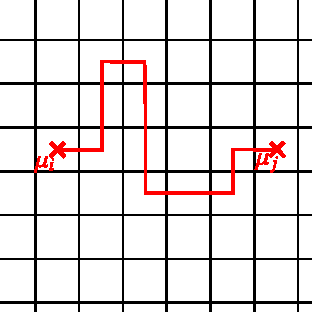
\includegraphics{disorder2.pdf}
  \caption{$a,b$の和をとってしまった後での無秩序演算子の様子。赤で表した経路は対称性欠陥$\eta$を表している。つまり、赤の線と交わっているリンクは反強磁性になっている。$\mu$演算子は$\eta$の端のプラケットに配置されている。}
  \label{fig:disorder2}
\end{figure}

\appendix
\section{計算}
\label{sec:calculation}
まず式\eqref{dualK}を導出しよう。
\begin{align}
  \frac{\sinh K}{\cosh K}=\tanh K = e^{-2\Kt}
  \label{KKt}
\end{align}
のとき、両辺の逆数をとって
\begin{align}
  \frac{\cosh K}{ \sinh K} = e^{2\Kt}
\end{align}
を得る。これらを引き算して
\begin{align}
  \frac{\cosh K}{\sinh K}-\frac{\sinh K}{\cosh K}=e^{2\Kt}-e^{-2\Kt}=2\sinh 2\Kt.
\end{align}
左辺を変形して
\begin{align}
  (\text{左辺})=\frac{\cosh^2K-\sinh^2 K}{\sinh K \cosh K}=\frac{1}{\frac{1}{2}\sinh 2K}
\end{align}
となる。したがって
\begin{align}
  \sinh 2K \sinh 2\Kt =1
\end{align}
を得る。これは式\eqref{dualK}である。

次に式\eqref{Zelltemp}を導出しよう。次のような変形を考える。
\begin{align}
  \sinh 2K = 2\cosh K \sinh K = 2 \cosh^2 K \tanh K =2\cosh^2 K e^{-2\Kt}.
\end{align}
最後の変形では\eqref{KKt}の関係を用いた。この式から
\begin{align}
  \cosh^2 K = \frac12 \sinh 2K e^{2\Kt}
\end{align}
を得るので、両辺の平方根をとって
\begin{align}
  \cosh K = \frac{1}{\sqrt{2}}\sqrt{\sinh 2K} e^{\Kt}
\end{align}
を得る。これと\eqref{KKt}を$2\cosh K (\tanh K)^c$に代入して
\begin{align}
  2\cosh K (\tanh K)^c
  =\sqrt{2\sinh 2K}e^{\Kt -2\Kt c}
  =\sqrt{2\sinh 2K}e^{\Kt (-1)^c}
\end{align}
を得る。これは式\eqref{Zelltemp}である。ここで$c=0,1$の場合に成り立つ恒等式
\begin{align}
  1-2c=(-1)^c
\end{align}
を用いた。
\printbibliography
\end{document}